%Template Rapport .tex créé par BALLEJOS Lilian

\documentclass[12pt,french]{article} %ajouter draft pour voir débordement
\usepackage[utf8]{inputenc}
\usepackage[T1]{fontenc}
\usepackage{lmodern}
%règles mes marges et format papier
\usepackage[a4paper,hmargin=2cm,vmargin=2cm]{geometry} %modif marge et formet
\usepackage{amsmath, amssymb, amsthm}
\usepackage{fancyhdr} %pour les entêtes et bas de page
\usepackage{lastpage} %pour numéroter les pages charge la derniere page
\usepackage{graphicx} %pour inclure des img
\usepackage{dsfont}
\usepackage{float} %pour le placement des figures
\usepackage{hyperref} %pour mettre des liens hypertext
\usepackage{calc} %permet de calculer les marges pour encadrer les textes
\usepackage{color, xcolor} %gère les couleurs
\usepackage{babel}
\usepackage{listings} %pour afficher le code annexe

%pour afficher le code de manière esthétique
\lstset{
  aboveskip=3mm,
  belowskip=-2mm,
  backgroundcolor=\color{white},
  basicstyle=\footnotesize,
  breakatwhitespace=false,
  breaklines=true,
  captionpos=b,
  commentstyle=\color{red},
  deletekeywords={...},
  escapeinside={\%*}{*)},
  extendedchars=true,
  framexleftmargin=16pt,
  framextopmargin=3pt,
  framexbottommargin=6pt,
  frame=tb,
  keepspaces=true,
  keywordstyle=\color{blue},
  language=C,
  literate=
  {²}{{\textsuperscript{2}}}1 {⁴}{{\textsuperscript{4}}}1
  {⁶}{{\textsuperscript{6}}}1
  {⁸}{{\textsuperscript{8}}}1
  {€}{{\euro{}}}1 {é}{{\'e}}1 {è}{{\`{e}}}1 {ê}{{\^{e}}}1 {ë}{{\¨{e}}}1
  {É}{{\'{E}}}1 {Ê}{{\^{E}}}1 {û}{{\^{u}}}1 {ù}{{\`{u}}}1 {â}{{\^{a}}}1
  {à}{{\`{a}}}1 {á}{{\'{a}}}1 {ã}{{\~{a}}}1 {Á}{{\'{A}}}1 {Â}{{\^{A}}}1
  {Ã}{{\~{A}}}1 {ç}{{\c{c}}}1 {Ç}{{\c{C}}}1 {õ}{{\~{o}}}1 {ó}{{\'{o}}}1 
  {ô}{{\^{o}}}1 {Õ}{{\~{O}}}1 {Ó}{{\'{O}}}1 {Ô}{{\^{O}}}1 {î}{{\^{i}}}1
  {Î}{{\^{I}}}1 {í}{{\'{i}}}1 {Í}{{\~{Í}}}1,
  morekeywords={*,...},
  numbers=left,
  numbersep=10pt,
  numberstyle=\tiny\color{black},
  rulecolor=\color{black},
  showspaces=false,
  showstringspaces=false,
  showtabs=false,
  stepnumber=1,
  stringstyle=\color{gray},
  tabsize=4,
}
%%%%%

%Personalisation En tête
\pagestyle{fancy}
\renewcommand\headrulewidth{1pt}
%permet d'aumenter tailler header pour mettre image (31pt ici)
\setlength{\headheight}{31pt}
\fancyhead[L]{Simulation - F2}
\fancyhead[C]{
\includegraphics[scale=0.2]{header.png}}
\fancyhead[R]{Lab \#3 - Simu PI \\ \& Conf Intervals}
\renewcommand\footrulewidth{1pt}
\fancyfoot[L]{BALLEJOS Lilian}
\fancyfoot[C]{\thepage/\pageref{LastPage}}
\fancyfoot[R]{2022/2023}
%Fin personalisation En Tête


\begin{document}

\begin{titlepage} %page d'acceuil

  
  
\includegraphics[scale=0.6]{isima.png}
  \hspace*{\stretch{1}}%espace horizontal entre les 2 images
  
\includegraphics[scale=0.10]{decoration.jpg}
  
  \vspace*{2.5cm} %espace de 2.5cm en dessous des images
  
  \begin{center}\huge
    \textbf{Rapport TP Simulation} 
    
    \textbf{Lab \#3 - Simu PI \& Conf Intervals}
  \end{center}
  
  \hrule %trait horizontal
  
  \begin{center}
    \Large BALLEJOS Lilian
    
    \large
    ISIMA INP Deuxième année
    
    Spécialité F2
    
    Année Universitaire 2022/2023
  \end{center}
  
  \begin{center}
    %créer une boite ou mettre l'image qui fait la largeur de la page
    \makebox[\textwidth]{
\includegraphics[width=\paperwidth]{garde.png}}
  \end{center}
  
  \vspace*{2cm} 
  
  \begin{flushright}\footnotesize %a droite
    Enseignant référant: Mr David HILL
    
    Date du rendu: 31 octobre 2022
    
    Date de la dernière modification: \today 
    %permet d'afficher la date ou je code actuellement (\today)
    
  \end{flushright}
  
  \begin{flushleft}\small %a gauche
    \textbf{ISIMA INP}
    \footnotesize
    
    1 rue de la Chebarde - TSA 60125 - CS 60026 - 63178 Aubière CEDEX
    
    Tel: 04 73 40 50 00
    
    Site web: \href{https://www.isima.fr/}{isima.fr}\newline	
  \end{flushleft}
\end{titlepage}	


%Ma table des Matières !
%permet de renommer 'table des matières' en sommaire
\renewcommand{\contentsname}{Table des Matières}
\normalsize\tableofcontents %place la table des matières

\bigskip

\section*{Introduction}



\subsection*{Quelques remarques sur le fichier .c}

Les commentaires \textbf{/**/} sont voués à être supprimés Ils sont ici pour rendre l'exécution du main plus lisible et ne pas biaiser les tirages aléatoires en enchainant des tirages.

\bigskip

La compilation s'effectue via un \textbf{Makefile}.

\bigskip

Liste des fichiers fournit pour ce TP:
\begin{itemize}
	\item mt.c
	\item mt.h
	\item makefile
	\item tp3\_ballejos.c
	\item tp3\_ballejos.pdf
\end{itemize}

\bigskip

J'ai réutilisé lors de ce TP les fonctions "MT" de génération de nombre aléatoire de Matsumoto que vous pouvez retrouver \href{http://www.math.sci.hiroshima-u.ac.jp/m-mat/eindex.html}{\underline{ici}}.


\newpage

\section{Exercice 1: Création d'une fonction qui approche la valeur de PI}

\subsection{Explication}

Nous allons tout d'abord commencer par créer une fonction nommée \textbf{simPi()} qui approche la valeur de $\pi$. Pour cela nous faisons la méthode de Monte-Carlo. La fonction prend en argument $n$ nombre de point à tirer dans un quart de cercle du cercle d'unité et en comptant la proportion présente dans le cercle on arrive à retrouver une valeur approximative de $\pi$ !

\subsection{Résultats}

On remarque pour le moment que plus on augmente le nombre de tirage de point plus on approche une meilleure valeur de $\pi$ ! 

\begin{figure}[H]
	\centering
	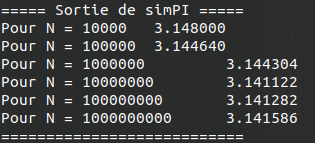
\includegraphics[scale=0.7]{exo1-1.png}
	\caption{Sortie de simPi() avec différents nombre de tirage}
\end{figure}

On remarque tout de même qu'avec 1 milliard de tirage on arrive seulement à atteindre les 4 premiers décimales de $\pi$ ! Nous pouvons surement trouver une meilleure méthode !

\section{Exercice 2: Obtention de PI par la moyenne}

\subsection{Explication}

Une autre solution pourrait être d'appeler plusieurs fois la fonction simPi() et de faire la moyenne de toutes les sorties !
Ainsi on a maintenant 2 paramètres qui sont le nombre de point tiré ainsi que le nombre de fois qu'on appelle simPi().
Voyons maintenant si on obtient des résultats plus intéressant.

\subsection{Résultats}

\begin{figure}[H]
	\centering
	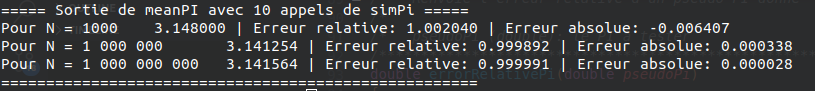
\includegraphics[scale=0.6]{exo2-1.png}
	\caption{Sortie de meanPI() avec 10 appels de simPi()}
\end{figure}


On remarque que l'erreur absolue tend de plus en plus vers 0 alors que l'erreur relative elle tend de plus en plus vers 1 ce qui est très bon signe.
Testons maintenant avec 40 appels de simPi()

\begin{figure}[H]
	\centering
	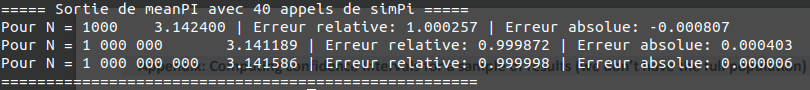
\includegraphics[scale=0.6]{exo2-2.png}
	\caption{Sortie de meanPI() avec 40 appels de simPi()}
\end{figure}

En plus de remarquer que mon ordinateur souffre de tirer 40 fois 1 milliards de point on peut aussi voir que les erreurs sont de plus proche de 0 et de 1 ce qui implique un bien meilleur pseudo PI approché.


\section{Exercice 3: Intervalle de confiance avec la moyenne de PI}

\subsection{Explication}

Nous allons maintenant maintenant effectuer un intervalle de confiance de notre $\pi$ simulé en calculant tout d'abord un estimateur non biaisé puis un l'intervalle.

\subsection{L'estimateur}

J'ai d'abord crée une nouvelle fonction \textbf{meanPiWithArray} qui effectue le même comportement que \textbf{meanPi} mais stocke aussi dans un tableau en argument toutes les sorties de $\pi$ ayant servi pour la moyenne. Ces valeurs vont nous servir à calculer l'estimateur à l'aide de cette formule:

\begin{figure}[H]
	\centering
	\begin{align}
		\overline{X}(n) = \sum_{i = 1}^{n} X_{i} / n \\
		S^{2}(n) = \frac{\sum_{i = 1}^{n} [X_{i} - \overline{X}(n)]^{2}}{n - 1}
	\end{align}
	\caption{Formule pour calculer l'estimateur} 
\end{figure}

C'est la fonction \textbf{EstimateWithoutBiasPi} qui retourne la valeur de l'estimateur.

\subsection{Calcul de R}

Après avoir calculé l'estimateur de notre pseudo $\pi$ il faut calculer R et pour cela la fonction \textbf{CalculR} entre en jeu.

Cette fonction retourne la valeur de R avec la formule suivante :

\begin{figure}[H]
	\centering
		$R = t_{n-1, 1-\frac{\alpha}{2}} * \frac{\sqrt{S^{2}(n)}}{n}$
	\caption{Formule pour calculer R} 
\end{figure}

Il faut remarquer que j'ai fourni dans mon code seulement les 30 premières valeurs de $t_{n-1, 1-\frac{\alpha}{2}}$. Ainsi il ne sera pas possible de calculer un intervalle avec plus de 30 appels de simPi().

\subsection{Calcul de l'intervalle de confiance}

Enfin avec la fonction \textbf{showConfidenceInterval} il nous suffit d'appeler dans l'ordre la fonction meanPiWithArray puis EstimateWithoutBiasPi et enfin CalculR pour avoir notre intervalle de confiance. J'ai juste à afficher dans le terminal l'intervalle en soustrayant et additionnant $R$ à la valeur du pseudo $\pi$ calculé.

\subsection{Résultat}

Voyons maintenant les résultats obtenus

\begin{figure}[H]
	\centering
	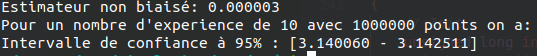
\includegraphics[scale=0.6]{exo3-0.png}
	\caption{Sortie de showConfidenceInterval avec 1 million de point et 10 appels de simPi}
\end{figure}

Avec 1 million de point et 10 appels de simPi on remarque l'intervalle est concluant mais peut être mieux

\begin{figure}[H]
	\centering
	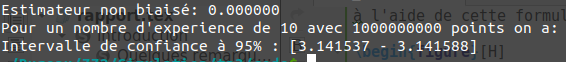
\includegraphics[scale=0.6]{exo3-1.png}
	\caption{Sortie de showConfidenceInterval avec 1 milliard de point et 10 appels de simPi}
\end{figure}

Avec 1 milliard de point et 10 appels de simPi le "printf lf" de \textit{stdlib.h} n'est pas suffisant pour afficheur l'estimateur tant il est petit ! L'intervalle est lui bien plus précis !

\begin{figure}[H]
	\centering
	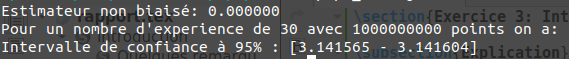
\includegraphics[scale=0.6]{exo3-2.png}
	\caption{Sortie de showConfidenceInterval avec 1 milliard de point et 30 appels de simPi}
\end{figure}

Enfin, avec 1 milliard de point et 30 appels de simPi on obtient des résultats moins précis que pour 10 appels ce qui n'est pas un résultat attendu.

Il semble que faire la moyenne avec beaucoup de valeur n'est la meilleure stratégie pour obtenir un meilleur intervalle ce confiance.


\listoffigures

\end{document}


